\chapter{In-silico Simulations}

\section{Implementation} 

In this work we used Python as an implementation tool. Here we used the libraries Numpy and Matplotlib, whereas the former is a free powerful scientific computing tool. It is equipped with an optimized linear algebra packages as well as module to generate random events. The latter is a presentation library which we used to present our performance tests. 

In the beginning we generated a random matrix using the module random from Numpy where it generated an array of zeros and ones uniformally distributed. 

We wrote pieces of code, these are, an implementation of IHT and its modification NHIT, also some tests on it. The other is an implementation of BIHT and also accompanied with some tests. 


We used various functions in Numpy we conducted the calculations and the iteration in the algorithm. In some occasions we produced our own functions as to help in the calculations.   


We used the computing infrastructure \textbf{Colab} offered by Google as a running server for our code and experiments. 

Next we present some segments of the code and its output. A full and documented code is available in the appendix.   

Here is an example of a matrix $A^{4\times 9}$ and a sparse vector $x^{9\times1}$ with sparsity $d = 2$ and also the measurement vector y, where the matrix $ A $ is generated randomly as well as x.  


\vspace{5mm}

$ A =  \begin{bmatrix}
0 & 0 & 1 & 0 & 1 & 1 & 0 & 1 &0 \\
1 & 1 & 1 & 0 & 1 & 1 & 0 & 0 &0 \\
1 & 0 & 0 & 0 & 1 & 0 & 0 & 1 &0 \\
0 & 1 & 0 & 0 & 0 & 1 & 1 & 1 &1 \\
\end{bmatrix}$,  \quad  $ x = [0, 1, 0, 0, 0, 1, 0, 0, 0]^{T} $  and $y = \begin{bmatrix}
1\\
1\\
0\\
1
\end{bmatrix}$
\vspace{5mm}
The first column of the matrix A above reads as the first individual is tested in the tests 2 and 3 but not tested in the first test and the last test, whereas the vector y tells us that the first ,second and fourth tests are positive which implies that at least one those participated in these tests is infected. 



Here is an example of the basic iterative threshold algorithm put to action applied on A, y and with 100 iterations

\vspace{5mm} 
$ A =  \begin{bmatrix}
1 & 1 & 0 & 0 & 0 & 1 & 1 & 0 &1 \\
0 & 0 & 1 & 0 & 0 & 1 & 1 & 1 &0 \\
1 & 0 & 1 & 1 & 1 & 0 & 1 & 0 &0 \\
1 & 0 & 1 & 0 & 1 & 0 & 1 & 0 &0 \\
\end{bmatrix}$,  \quad , $y = \begin{bmatrix}
0\\
1\\
1\\
1
\end{bmatrix}$
and $ x = [0, 0, 1, 0, 1, 0, 0, 0, 0]^{T} $ 

\vspace{5mm}
the result of iteration is the vector $ x^* = [0, 0, 1, 1, 1, 0, 1, 1, 0]^{T} $ 
\vspace{5mm}

Let us define an operator, $\sigma$  , which is in simple words the difference between two vectors index by index, i.e. it counts the differences. 

Here is a histogram of the differences of 3000 vectors with $ n = 14, m= 7, d = 2 $ and their recovered vectors using the basic thresholding algorithms with 1000 iterations. 
\vspace{5mm}
\begin{figure}[H]
	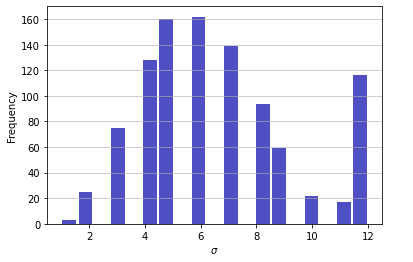
\includegraphics[height=8cm, width=8cm]{images/hamming_basic}
	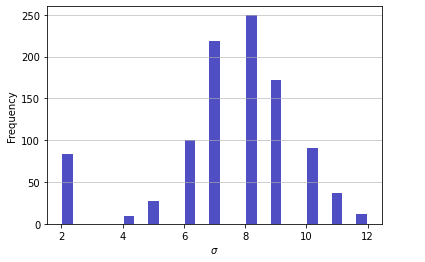
\includegraphics[height=8cm, width=8cm]{images/n_hamming}
	\caption{$ \sigma $ between the vectors and their recovered using the basic threshold iterative algorithm (left) and the normalized threshold iterative algorithm (right)for 3000 vectors}
\end{figure}
%It can be seen that the differences trend is almost the natural distribution. Where as these results are considered as desired but in the above example we relaxed the constraints. In the next section we focus on (BIHT) as our main target of tests.

Now lets test the probability of exact recovery of the algorithm. We ran a 100 simulation of a sample of 100 ($ n =100 $) and we took different values of $ m $ (tests) each time, that is we increase $ m $ be 5 up to $ n $.    

\begin{figure}[H]
	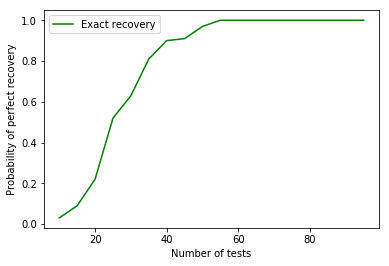
\includegraphics[height=8cm, width=8cm]{images/basic_exa}
	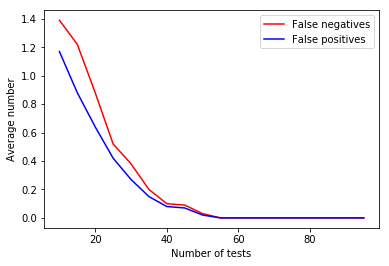
\includegraphics[height=8cm, width=8cm]{images/basic_false}
	\caption{This figure shows the probability of exact recovery (left) and  the average of false positive and false negatives vs the number of tests m (right), with number of individuals  = 100 and the number of defectives 2}
\end{figure}

\section{Binary iterative hard thresholding performance}

In this section we apply some tests on the binary iterative thresholding algorithm. We chose this algorithms as it is convenient to work with, because of its binary nature, as well as its robustness and stability which is shown in \cite{biht}. 

Primarily, we are testing the probability of exact recovery, specificity (false positive), and sensitivity (false negative). We will also include the $ \sigma $ test mentioned above. 

We run a number of simulations, in each of which we change the number of tests $ m $ according to the number individuals to be tested. 

The following graphs represent results from simulating the test 100 times with different number of individuals participating in the test.  

It is important that in both of following results the gradient descent (step size)  is kept fixed at $ \mu = 0.001 $

 \begin{figure}[H]
	%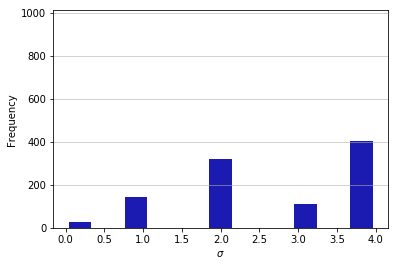
\includegraphics[height=8cm, width=8cm]{images/sigma_biht}
	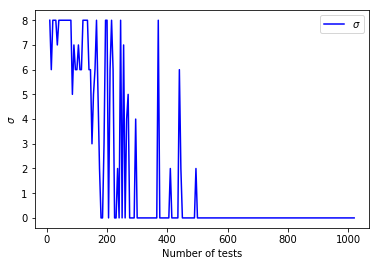
\includegraphics[height=8cm, width=8cm]{images/sigmavsm}
	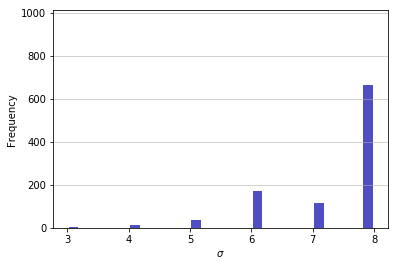
\includegraphics[height=8cm, width=8cm]{images/sigma_512}
	\caption{$ \sigma $ vs the number of tests $ m $ on the right and $ \sigma $ between the vectors and their recovered using the binary threshold iterative algorithm (BIHT) simulated 1000}
	\label{sigma}
\end{figure}
\begin{figure}[H]
	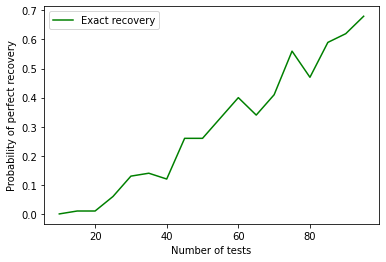
\includegraphics[height=8cm, width=8cm]{images/index1}
	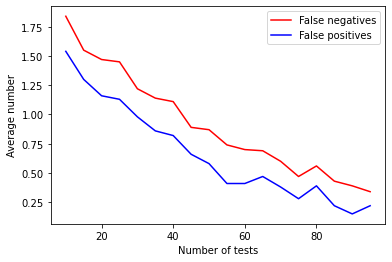
\includegraphics[height=8cm, width=8cm]{images/index}
	\caption{This figure shows the probability of exact recovery (left) and  the average of false positive and false negatives vs the number of tests m (right), with number of individuals  = 512 and the number of defectives 2, with $ \mu = 0.001 $}
	\label{exat}
\end{figure}

%\begin{figure}[H]
%	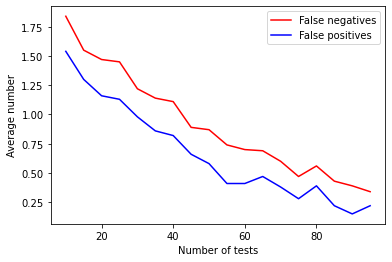
\includegraphics[height=9cm, width=8cm]{images/index}
%	\caption{This figure shows the average of false positive and false negatives vs the number of tests m, with number of individuals  = 100 and the number of defectives 2}
%\end{figure}

Next we increase the number of individuals and watch the three indicators mentioned above, taking the same test for 512, and 1024 individuals also keeping the number defectives low. 

\begin{figure}[H]
	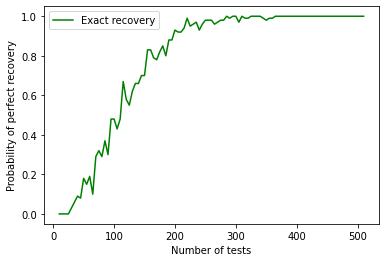
\includegraphics[height=8cm, width=8cm]{images/512ex}
	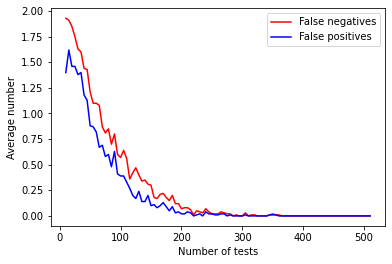
\includegraphics[height=8cm, width=8cm]{images/512fal}
	\caption{This figure shows the probability of exact recovery (left) and  the average of false positive and false negatives vs the number of tests m (right), with number of individuals  = 512 and the number of defectives 2, with $ \mu = 0.001 $}
	\label{exat1}
\end{figure}

Now we change the gradient descent $ \mu $, we set to $ 0.1 $ which relatively bigger than what chose first $ 0.001 $.

\begin{figure}[H]
	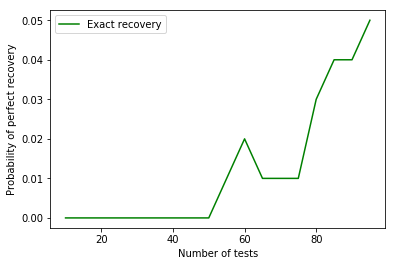
\includegraphics[height=8cm, width=8cm]{images/exa_mu}
	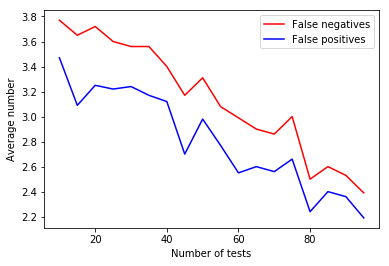
\includegraphics[height=8cm, width=8cm]{images/fal_mu}
	\caption{This figure shows the probability of exact recovery (left) and  the average of false positive and false negatives vs the number of tests m (right), with number of individuals  = 512 and the number of defectives 2, here $ \mu = 0.1 $}
	\label{mu}
\end{figure}


\subsection{Notes on the results of the BIHT simulation} 


\begin{itemize}
	\item The $ \sigma $ test that we run on the algorithm roughly tells us the convergence of the algorithm, where as we can see in  \ref{sigma} that with simulating the recovery 1000 times, most the $ \sigma $s are around $ 2d $, being the number of defectives. 
	
	\item The exact (perfect) recovery probability increases with increasing the number of tests $ m $,  but it noticed that from \ref{exat} on the left, \ref{exat1}, with the increase of $ n $, the algorithm starts to be more efficient, and it gives an exact recovery of probability of 1 earlier.    
	\item The false-positives and false-negative starts to fall sharply with increase of but with number of tests approaches certain point they being to stabilize at 0 \ref{exat1} on the right. 
	
	\item As $ \mu $ being very small the curves starts to be smother \ref{exat1} and \ref{mu}.    
\end{itemize}
 \section{Python code}
 
 The codes that are used in this thesis are available at: \href{https://github.com/KhalidOmer/School_thesis/tree/main}{github.com/KhalidOmer}
 
 
 The file README.md contains a brief description of the codes and what they do as well as how to
 run them.